\section{预算与结果评价}
\label{sec:bo-budget}

循环总要结束。本节回答最后几个问题：预算究竟应当怎样计算，什么时候停止，交出什么，这个结果好到什么程度，以及哪些结论有理论保证。这些问题放在一起，是因为比较方法时必须固定同一套口径：搜索域、可用信息和预算。

\subsection{评价成本}
\label{sec:bo-cost}

不同位置的运行代价可能差别很大，比如某个参数越大，仿真越慢。一种常见的调整是除以预测成本$\widehat{c}(\bm{x})$，选单位成本的改进最大的点：
\begin{equation}
 \alpha_t^{\mathrm{cost}}(\bm{x})=\frac{\mathrm{EI}_t(\bm{x})}{\widehat{c}(\bm{x})}.
 \label{eq:bo-cost-ei}
\end{equation}
这只是一种特定的预算策略，它不自动最优地分配剩余总预算。下面的小例子说明这一点。剩余预算是$9$，候选A成本$1$、预期收益$2$，候选B成本$9$、预期收益$16.2$。单位成本的收益分别为
\[
 2,\qquad1.8.
\]
按单位成本选A，用掉$1$后，剩余$8$不够运行B，总收益只有$2$；一开始就选B，总收益为$16.2$。贪心比值没有考虑“预算够不够下一个”。

时间也要分开算。评价次数少不等于总耗时短。表~\ref{tab:bo-time}区分三种常被混用的时间。若一次评价只要$1$秒，贝叶斯优化的内层计算可能远超评价本身，这时随机搜索更快；若一次评价要$1$小时，每轮花$1$分钟做选点几乎没有成本。比较方法时只比较外层迭代数，等于默认了内层计算不要钱。

\begin{BookInlineTable}
 \centering
 \caption{三种时间口径，$c_i$是第$i$次评价的耗时，$a_i$是第$i$轮算法计算的耗时，$q$是并行的机器数。}
 \label{tab:bo-time}
 \begin{tabular}{ll}
 \toprule
 口径&计算方式\\
 \midrule
 串行总耗时&$\sum_i(c_i+a_i)$\\
 并行等待时间&约$\sum_i c_i/q$，耗时不等时更长\\
 算法自身计算时间&$\sum_i a_i$，高斯过程每轮约$O(t^3)$\\
 \bottomrule
 \end{tabular}
\end{BookInlineTable}

\subsection{停止与推荐}
\label{sec:bo-stopping}

最直接的停止条件是预算耗尽，这不需要任何模型。也可以在采集分数很小时提前停止，例如$\max_{\bm{x}}\mathrm{EI}_t(\bm{x})$低于一个阈值。这种停止依赖两件事：代理是否可信，以及内层求解是否找到了采集函数的最大点。第~\ref{sec:bo-model-specification}节中$\ell=3$的模型在$x=6$处方差极小，据此计算的EI也很小，算法就会在没有真正探索的情况下停下来。

推荐规则要在运行前说定。无噪声时可以返回已评价的最好点，贯穿例中就是$\widehat{x}_6=6$。含噪时，已评价的最好读数可能只是运气，通常用后验均值提出候选，例如选$\min_{\bm{x}}m_T(\bm{x})$的位置，再用预留的预算在候选处复测。最后报告采用的推荐规则，以及推荐值的不确定性，不只报告一个数字。

\subsection{推荐误差}
\label{sec:bo-regret}

交出$\widehat{\bm{x}}_T$后，自然要问它离最好的结果有多远。记$f^\star=\inf_{\bm{x}\in\bm{C}}f(\bm{x})$，用\term{简单遗憾}（simple regret）$f(\widehat{\bm{x}}_T)-f^\star$衡量最终结果，也就是终端的推荐误差。

另一个常见的量是\term{累积遗憾}（cumulative regret）：
\begin{equation}
 R_T=\sum_{t=1}^T\bigl(f(\bm{x}_t)-f^\star\bigr).
 \label{eq:bo-cumulative-regret}
\end{equation}
它把每次评价相对$f^\star$的损失都算进去，适用于每次试验本身就有代价的场合，这种在线损失的完整讨论可参考\BookChapterRef{chap:partial-observation-exploration}{卷十第3章“部分观测、主动观测与探索”}。两者回答的问题不同：贝叶斯优化的目标是最后交一个好答案，探索阶段的差读数并不算损失。

贯穿例上的简单遗憾是
\[
 f(6)-f^\star\approx-1.0+1.029=0.029,
\]
这个差距来自算法只在整数候选上选点，而样条的最小点在$x\approx6.13$。

图~\ref{fig:bo-regret-curves}在贯穿例上比较贝叶斯优化和均匀随机搜索，共$15$次评价，都从相同的$3$个随机点出发。(a)是当前已评价的最好值相对$f^\star$的差，贝叶斯优化第$8$次之后基本为零，$15$次时平均差约$0.002$，随机搜索约$0.142$。(b)的累积损失两者差别小得多，分别约为$14.2$和$16.3$，因为贝叶斯优化在找到好的位置之后仍在探索其他区域。同一个方法，按不同的指标看，结论可能不同。

\begin{BookInlineFigure}
 \centering
 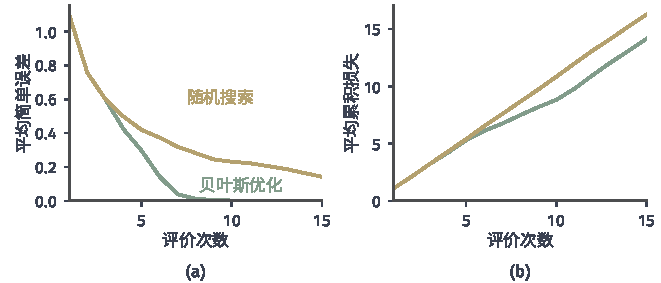
\includegraphics[width=112mm]{figures/05-optimization/05-stochastic-optimization/matplotlib/bo-regret-curves/figure.pdf}
 \caption{贯穿例上的两种误差，$200$组随机初始点的平均值。绿线是贝叶斯优化（$0.1$网格、EI），黄线是均匀随机搜索。(a)当前最好值相对$f^\star$的差；(b)累积损失~\eqref{eq:bo-cumulative-regret}。这是单个一维目标上的教学实验，不代表一般结论。}
 \label{fig:bo-regret-curves}
\end{BookInlineFigure}

\paragraph{不知道$f^\star$时}
贯穿例是人为构造的，$f^\star$可以直接算出。实际问题的最优值未知，就不能直接报告精确的推荐误差，能报告的只有依据明确的比较。可以用已知最优值的基准问题来测方法；可以用有效的下界，比如若$f$是$L$-Lipschitz的，且搜索域中每点到最近评价点的距离不超过$h$，则
\begin{equation}
 f^\star\geq\min_{i\leq T}f(\bm{x}_i)-Lh.
 \label{eq:bo-lipschitz-bound}
\end{equation}
这个不等式成立，因为最小点到某个评价点的距离不超过$h$，函数值的差不超过$Lh$。贯穿例中六个评价点的覆盖半径$h=1.5$，若取$L=2$，下界只有$-4$，松得多，可见这类下界常常只能给出保守的结论。还可以用独立的复核运行来比较候选，这能说明“比基线好多少”，不能说明“离最优多远”。

\subsection{保证的条件}
\label{sec:bo-guarantees}

贝叶斯优化有理论保证吗？可以说有，但条件比较具体。第~\ref{sec:bo-lcb}节留下的问题是：$\kappa_t$取多大，LCB才是有效的置信界？下面的定理针对有限搜索域。

\begin{theorem}[有限搜索域上的同时置信界]
\label{thm:bo-confidence}
设$\bm{C}$是有限集，$f$确实是高斯过程$F$的一个实现，读数噪声是相互独立的$N(0,\tau^2)$，$\tau\geq0$，且每个$\bm{x}_t$只依赖$\mathcal{D}_{t-1}$（可以再用与$F$独立的随机数）。对$\delta\in(0,1)$，令
\begin{equation}
 \beta_t=2\log\frac{\lvert\bm{C}\rvert\pi^2t^2}{6\delta}.
 \label{eq:bo-beta}
\end{equation}
则以至少$1-\delta$的概率，对所有$t\geq1$和所有$\bm{x}\in\bm{C}$，都有
\begin{equation}
 \lvert F(\bm{x})-m_{t-1}(\bm{x})\rvert\leq\sqrt{\beta_t}\,s_{t-1}(\bm{x}).
 \label{eq:bo-confidence}
\end{equation}
\end{theorem}

\begin{proof}
先建立高斯尾的上界。设$W\sim N(0,1)$，$c\geq0$。把积分变量写成$w=c+u$，有
\[
 \phi(c+u)=\phi(u)\,e^{-c^2/2-cu}\leq\phi(u)\,e^{-c^2/2},\qquad u\geq0.
\]
在$u\geq0$上积分，得$\mathbb{P}(W>c)\leq\frac12e^{-c^2/2}$，再由对称性，
\[
 \mathbb{P}(\lvert W\rvert>c)\leq e^{-c^2/2}.
\]

固定$t$和$\bm{x}$。给定$\mathcal{D}_{t-1}$时，$F(\bm{x})$服从$N(m_{t-1}(\bm{x}),s_{t-1}^2(\bm{x}))$。若$s_{t-1}(\bm{x})=0$，不等式~\eqref{eq:bo-confidence}必然成立；否则应用上界，
\[
 \mathbb{P}\bigl(\text{式~\eqref{eq:bo-confidence}对这一组}(t,\bm{x})\text{不成立}\mid\mathcal{D}_{t-1}\bigr)\leq e^{-\beta_t/2}.
\]
这个上界不依赖$\mathcal{D}_{t-1}$，所以对$\mathcal{D}_{t-1}$取期望后仍成立。

对所有$\bm{x}$和所有$t$作并集界。由式~\eqref{eq:bo-beta}，
\[
 e^{-\beta_t/2}=\frac{6\delta}{\lvert\bm{C}\rvert\pi^2t^2},
\]
于是失败概率不超过
\[
 \sum_{t=1}^\infty\sum_{\bm{x}\in\bm{C}}\frac{6\delta}{\lvert\bm{C}\rvert\pi^2t^2}
 =\sum_{t=1}^\infty\frac{6\delta}{\pi^2t^2}=\delta.
\]
最后一步用了$\sum_{t\geq1}1/t^2=\pi^2/6$。
\end{proof}

证明之所以能处理自适应选点，靠的是对每个$t$先以历史为条件，并对$\bm{C}$中全部点取并集，于是不管算法选哪个点，界都成立。代价是系数比单点区间大。$\lvert\bm{C}\rvert=9$，$\delta=0.1$时，
\[
 \sqrt{\beta_1}\approx3.16,\qquad\sqrt{\beta_{10}}\approx4.38,\qquad\sqrt{\beta_{100}}\approx5.33,
\]
都比单点$95\%$区间的$1.96$大得多，且随$t$缓慢增大。

有了同时置信界，LCB的单步损失立刻受控。令$\kappa_t=\sqrt{\beta_t}$，$\bm{x}_t$是$\mathrm{LCB}_{t-1}$的最小点，$\bm{x}^\star$是$f$的最小点。在式~\eqref{eq:bo-confidence}成立的事件上，
\[
 f(\bm{x}_t)\leq m_{t-1}(\bm{x}_t)+\kappa_ts_{t-1}(\bm{x}_t),
\]
而由$\bm{x}_t$的选取，
\[
 m_{t-1}(\bm{x}_t)-\kappa_ts_{t-1}(\bm{x}_t)\leq m_{t-1}(\bm{x}^\star)-\kappa_ts_{t-1}(\bm{x}^\star)\leq f^\star.
\]
两式相减，得到
\begin{equation}
 f(\bm{x}_t)-f^\star\leq2\kappa_ts_{t-1}(\bm{x}_t).
 \label{eq:bo-instant-regret}
\end{equation}
单步损失不超过所选位置的后验标准差的$2\kappa_t$倍，评价的位置不确定性越小，损失越小。

对式~\eqref{eq:bo-instant-regret}求和，再把后验标准差之和联系到\emph{最大信息增益}$\gamma_T$，就得到累积遗憾的上界：若$\tau>0$，$k(\bm{x},\bm{x})\leq1$，上述事件上对所有$T$，
\begin{equation}
 R_T\leq\sqrt{C_1T\beta_T\gamma_T},\qquad C_1=\frac{8}{\log(1+\tau^{-2})},
 \label{eq:bo-regret-bound}
\end{equation}
其中$\gamma_T$是在$T$个点上观测所能获得的最大信息增益。这一步的证明需要用到高斯信息量的链式分解和方差的求和估计，篇幅较长，读者可查阅GP-UCB方法的原始分析。对平方指数核和紧凸搜索域，$\gamma_T$随$T$只按$\log T$的多项式增长，所以$R_T/T\to0$。

这个结论的适用范围要说清楚。它要求$f$确实由所用的高斯过程产生、核和噪声方差已知、内层问题精确求解、搜索域有限；连续域需要额外的光滑性条件和离散化论证。它只对这种特定的GP置信界方法成立，不覆盖任意代理与采集函数的组合。常用的EI加上每轮重新估计超参数，就不在这个定理的范围内，模型失配和内层求解误差也都要另外检查。

表~\ref{tab:bo-claims}把几种容易混淆的说法分开。

\begin{BookInlineTable}
 \centering
 \caption{三种不同的主张。}
 \label{tab:bo-claims}
 \begin{tabular}{ll}
 \toprule
 主张&需要的条件\\
 \midrule
 单点后验可信区间&模型正确，点在观测前固定\\
 自适应的同时置信界&模型正确，并集界，系数随$t$增大\\
 有限预算找到全局最优&一般不成立，需要对$f$作额外假设\\
 \bottomrule
 \end{tabular}
\end{BookInlineTable}

最后一行值得多说一句。有限次评价只能在有限个点取值，两个点之间函数可以任意低，除非另有光滑性之类的假设，否则任何算法都不能保证找到全局最优。这也是概率模型的角色所在：它把这种假设明确写了出来，让我们知道结论依赖什么。
